% !Rnw weave = knitr
\documentclass[a4paper, french, 11 pt]{article}\usepackage[]{graphicx}\usepackage[]{xcolor}
% maxwidth is the original width if it is less than linewidth
% otherwise use linewidth (to make sure the graphics do not exceed the margin)
\makeatletter
\def\maxwidth{ %
  \ifdim\Gin@nat@width>\linewidth
    \linewidth
  \else
    \Gin@nat@width
  \fi
}
\makeatother

\definecolor{fgcolor}{rgb}{0.345, 0.345, 0.345}
\newcommand{\hlnum}[1]{\textcolor[rgb]{0.686,0.059,0.569}{#1}}%
\newcommand{\hlstr}[1]{\textcolor[rgb]{0.192,0.494,0.8}{#1}}%
\newcommand{\hlcom}[1]{\textcolor[rgb]{0.678,0.584,0.686}{\textit{#1}}}%
\newcommand{\hlopt}[1]{\textcolor[rgb]{0,0,0}{#1}}%
\newcommand{\hlstd}[1]{\textcolor[rgb]{0.345,0.345,0.345}{#1}}%
\newcommand{\hlkwa}[1]{\textcolor[rgb]{0.161,0.373,0.58}{\textbf{#1}}}%
\newcommand{\hlkwb}[1]{\textcolor[rgb]{0.69,0.353,0.396}{#1}}%
\newcommand{\hlkwc}[1]{\textcolor[rgb]{0.333,0.667,0.333}{#1}}%
\newcommand{\hlkwd}[1]{\textcolor[rgb]{0.737,0.353,0.396}{\textbf{#1}}}%
\let\hlipl\hlkwb

\usepackage{framed}
\makeatletter
\newenvironment{kframe}{%
 \def\at@end@of@kframe{}%
 \ifinner\ifhmode%
  \def\at@end@of@kframe{\end{minipage}}%
  \begin{minipage}{\columnwidth}%
 \fi\fi%
 \def\FrameCommand##1{\hskip\@totalleftmargin \hskip-\fboxsep
 \colorbox{shadecolor}{##1}\hskip-\fboxsep
     % There is no \\@totalrightmargin, so:
     \hskip-\linewidth \hskip-\@totalleftmargin \hskip\columnwidth}%
 \MakeFramed {\advance\hsize-\width
   \@totalleftmargin\z@ \linewidth\hsize
   \@setminipage}}%
 {\par\unskip\endMakeFramed%
 \at@end@of@kframe}
\makeatother

\definecolor{shadecolor}{rgb}{.97, .97, .97}
\definecolor{messagecolor}{rgb}{0, 0, 0}
\definecolor{warningcolor}{rgb}{1, 0, 1}
\definecolor{errorcolor}{rgb}{1, 0, 0}
\newenvironment{knitrout}{}{} % an empty environment to be redefined in TeX

\usepackage{alltt}
\usepackage[T1]{fontenc}
\usepackage[utf8]{inputenc}
\usepackage{lmodern}
\usepackage{textcomp}
\usepackage[french]{babel}
\usepackage{graphicx}
\usepackage{geometry}
\geometry{top=2cm, bottom=2cm}
\usepackage{hyperref}
\hypersetup{pdfborder=0 0 0}
\usepackage{epstopdf}
\usepackage{booktabs}
\usepackage[skip=0.5\baselineskip]{caption}
\usepackage[backend=biber, isbn=false, doi=false, url=false, eprint=false, citestyle=ext-authoryear, maxnames=5, hyperref=true]{biblatex}
\DeclareOuterCiteDelims{parencite}{\bibopenbracket}{\bibclosebracket}
\usepackage[french=quotes, csdisplay=true]{csquotes}
\usepackage{enumitem}
\usepackage{array}% dans le préambule
\setlength{\extrarowheight}{0,1cm}

\newcounter{rownumbers}
\newcommand\rownumber{\stepcounter{rownumbers}\arabic{rownumbers}}

\epstopdfDeclareGraphicsRule{.gif}{png}{.png}{convert gif:#1 png:\OutputFile}
\AppendGraphicsExtensions{.gif}
\usepackage{listings}
\usepackage{inconsolata}
\usepackage{appendix}
\renewcommand{\appendixpagename}{Annexes}
\renewcommand{\appendixtocname}{Annexes}

\addbibresource{Econometrie.bib}

\title{Les déterminants du salaire au Pays-Bas\\
\vspace{0,5cm}
{\normalsize Projet d'économétrie --- Département de Sciences Humaines et Sociales\\
\vspace{0,5cm}
École normale supérieure Paris-Saclay}}
\author{\normalsize Louis Bourges, Jean-Baptiste Lagrange-Dupuis et Luc Letonturier}
\date{\normalsize\today}
\IfFileExists{upquote.sty}{\usepackage{upquote}}{}
\begin{document}

\maketitle

\section*{Introduction}

Depuis Becker et sa théorie du capital humain en 1964, les travaux économiques visant à expliquer les différences de revenu entre les individus se sont multipliées. Becker a théorisé l’existence d’un calcul coût-avantage microéconomique, qui conduit les individus à arbitrer entre le coût d’une année supplémentaire d’études et le gain espéré à long terme \parencite{becker1964}. Mincer, une décennie plus tard, a enrichi cette approche en incluant l’expérience accumulée au cours des années de travail dans le capital humain \parencite{mincer1974}.

Dans notre étude, nous tenterons de mesurer les effets de ces variables mais aussi d’autres paramètres, à l’instar du genre, de la présence d’enfants, mais aussi des heures travaillées ou de l’âge. Nous nous baserons sur deux enquêtes du LISS\footnote{\textit{Longitudinal Internet studies for the Social Sciences}, les questionnaires sont administrées par Centerdata} menées aux Pays-Bas respectivement en mai 2022 et en septembre 2022. Il s’agira, après une régression classique permettant de comprendre l’influence des différentes variables, de tester la présence d’hétéroscédasticité dans le modèle et, le cas échéant, de la corriger ; de mener un test de Chow pour tenter d'identifier d'éventuels effets de “paliers” quant au lien entre salaire et éducation ainsi que de discuter de la présence d’endogénéité dans le modèle et des moyens à notre disposition pour la corriger. Nous replacerons notre travail dans le contexte de la littérature existante et discuterons aussi de ses limites.



\section{Présentation du modèle et de ses limites}

\subsection{Présentation des variables utilisées}

Nous avons sélectionné plusieurs variables au sein de l’enquête \textit{Work and Schooling} et de la base \textit{Background variables}. La variable \verb+education+, issue d’un recoupement de plusieurs variables, correspond au nombre d’années de scolarité et d’études achevée (c’est-à-dire ayant conduit à l’obtention d’un diplôme), ses valeurs sont comprises entre 0 (personne n’étant jamais allée à l’école) à 22.5 (personne titulaire d’un doctorat, sachant que la scolarité débute à l’âge de 4 ans aux Pays-Bas). La variable \verb+genre+ sépare la population en deux groupes : hommes et femmes, les autres identités de genre ayant été écartées car très peu nombreuses et ayant été jugées difficilement interprétables et \verb+age+ indique l’âge des enquêtés. La variable \verb+revenu+ prend en compte le revenu brut mensuel autodéclaré, que nous avons préféré au revenu net, plus dépendant des politiques fiscales et de redistribution. La variable \verb+heures+ correspond au nombre d’heures de travail effectuées en moyenne chaque semaine tandis qu’\verb+experience+ mesure l’ancienneté des salariés dans leur entreprise (en années) ; il est à noter qu’un licenciement ou une démission remet ce compteur d’expérience à zéro puisque c’est l’expérience dans l’entreprise actuelle. Enfin, \verb+nbenfants+ indique le nombre d’enfants présents dans le foyer. 

\subsection{Détection et correction de l’hétéroscédasticité}





Afin de vérifier la présence ou non d’hétéroscédasticité au sein de notre modèle, nous avons réalisé les deux variantes du test de Breusch-Pagan (avec un test de Fisher et avec un test du rapport de vraisemblance) que nous avons également vérifié manuellement pour nous assurer d’obtenir les mêmes valeurs (p-value). Tous concordent et corroborent la présence d’hétéroscédasticité, qui est par ailleurs observable graphiquement : la répartition des résidus en fonction des données prédites n’est pas homogène et l’on observe une forte variabilité de ces résidus en fonction de certaines variables du modèle, notamment la variable heures (\bsc{Figure} \ref{fig:hetero}) où la dispersion semble être plus forte entre 30 et 40 heures qu’avant ou après. Avec le test de Breusch-Pagan avec le rapport de vraisemblance, dont nous avons vérifié les résultats via la commande \verb+bptest()+, nous obtenons une statistique de 75.6 et une p.value de \ensuremath{2.9\times 10^{-14}}, qui nous permet de rejeter l’hypothèse nulle au seuil significatif de 0,01. 

\begin{figure}[h]
\center
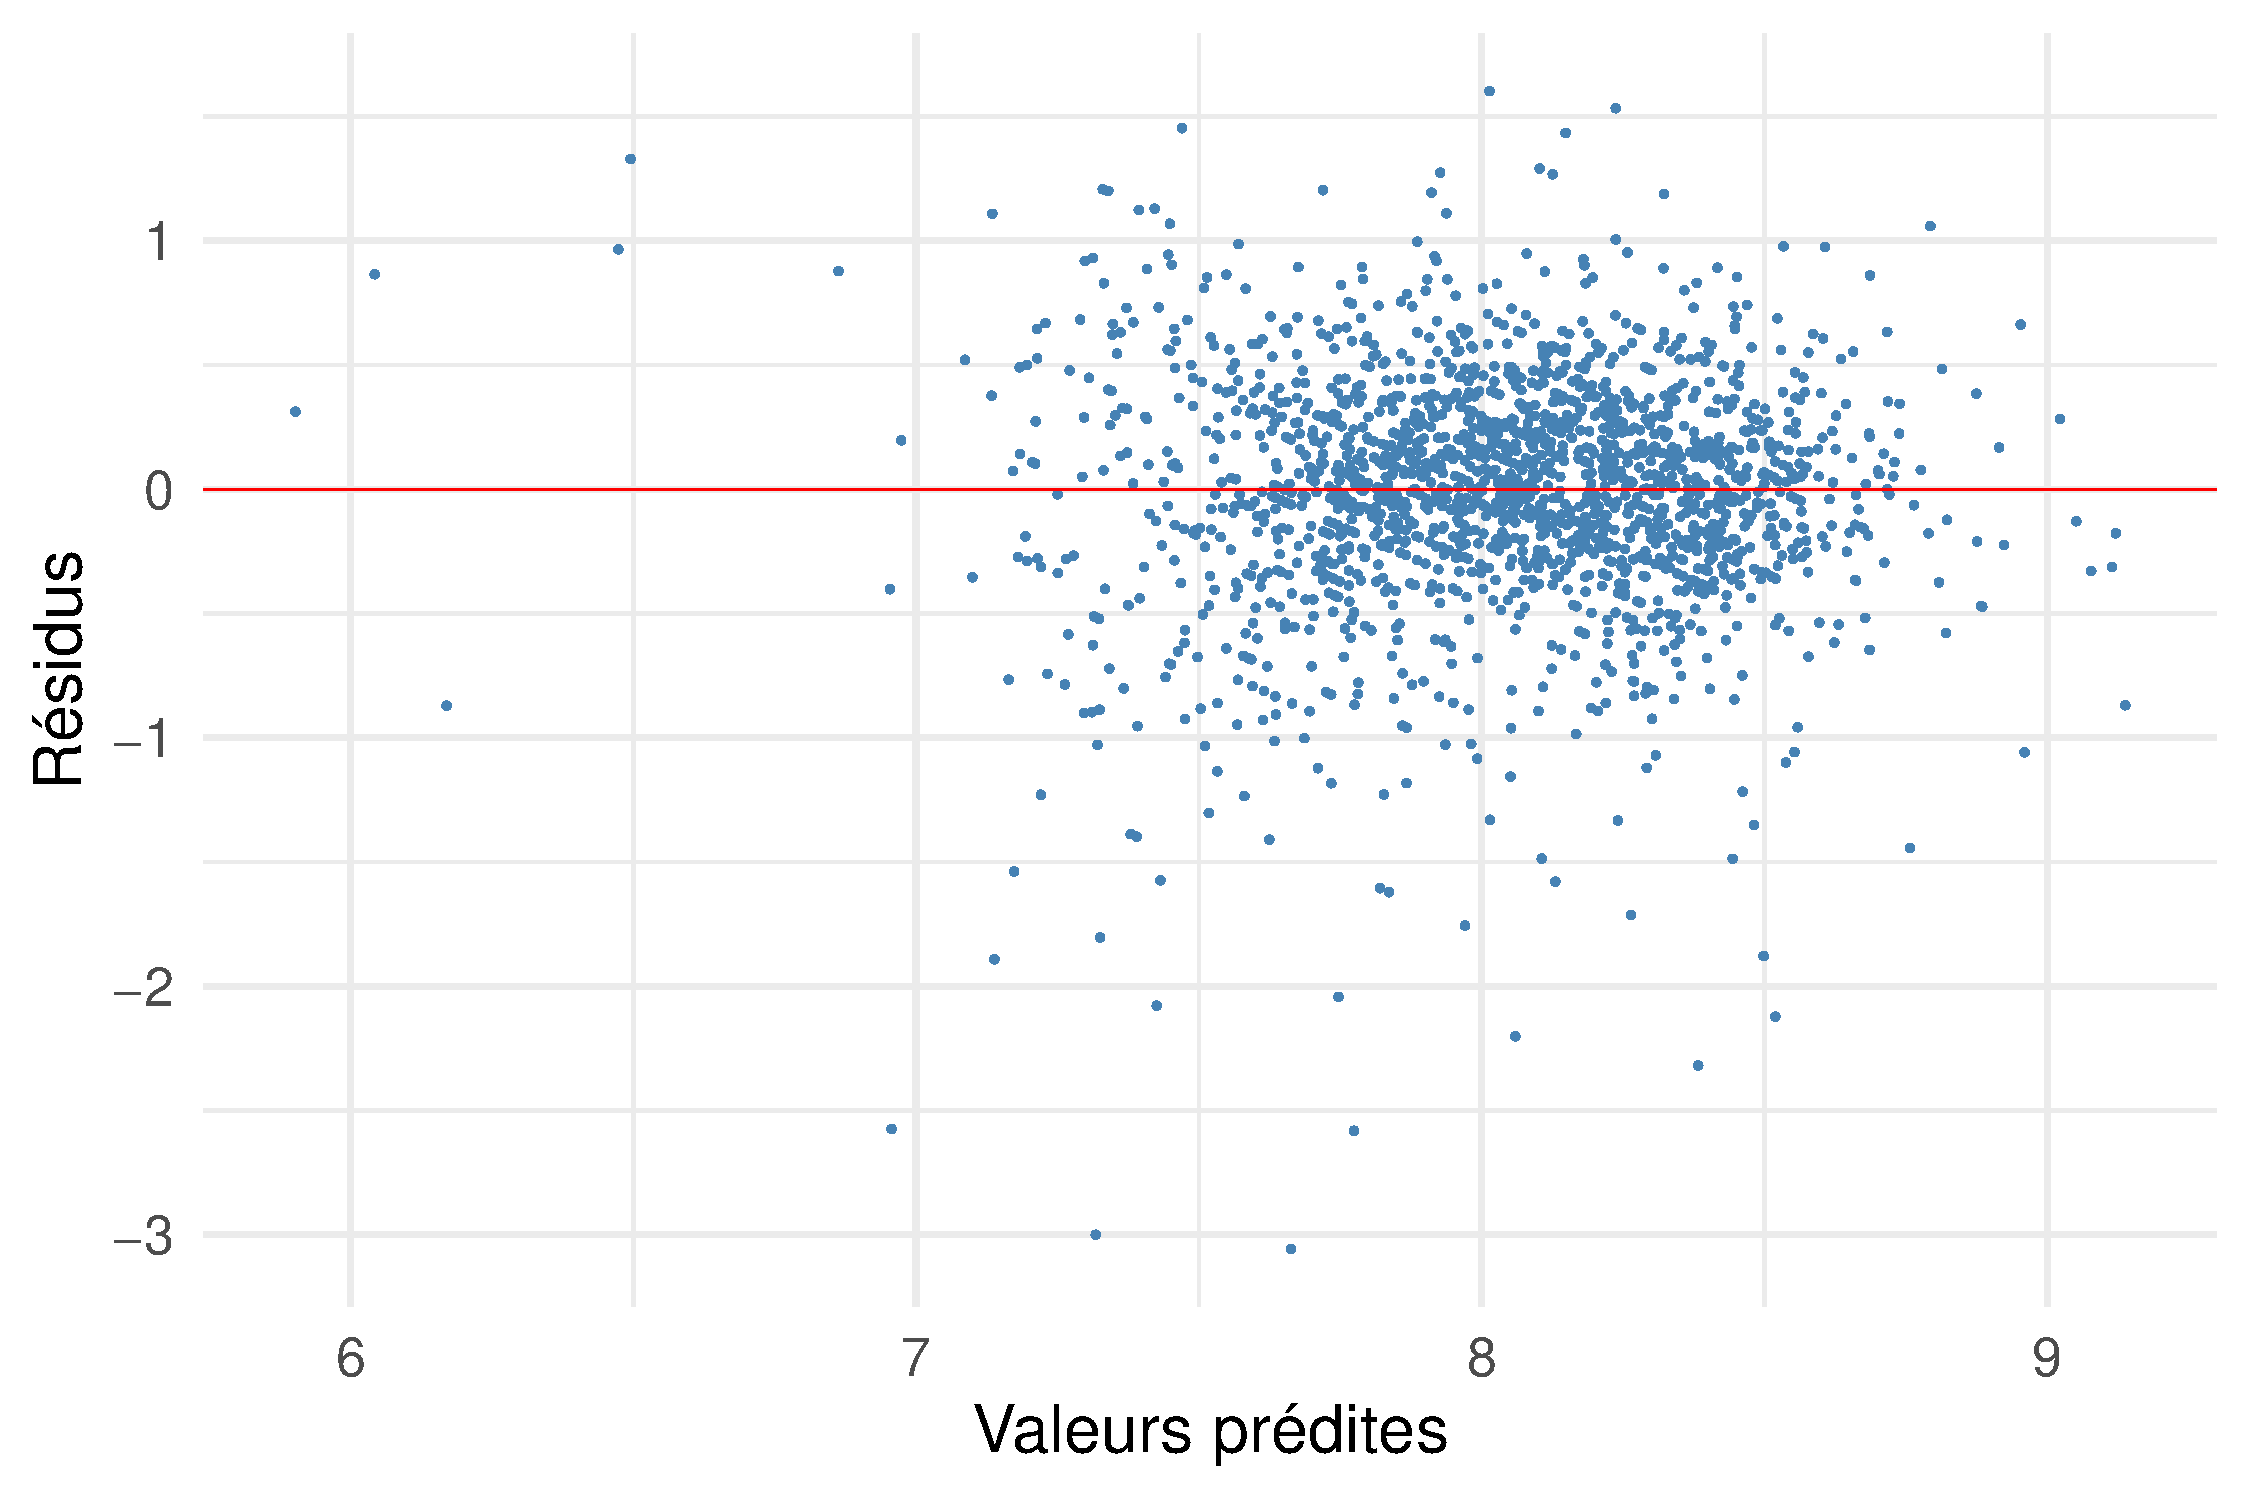
\includegraphics[width=0.49\linewidth]{figure/plot_hetero_fitted.pdf}
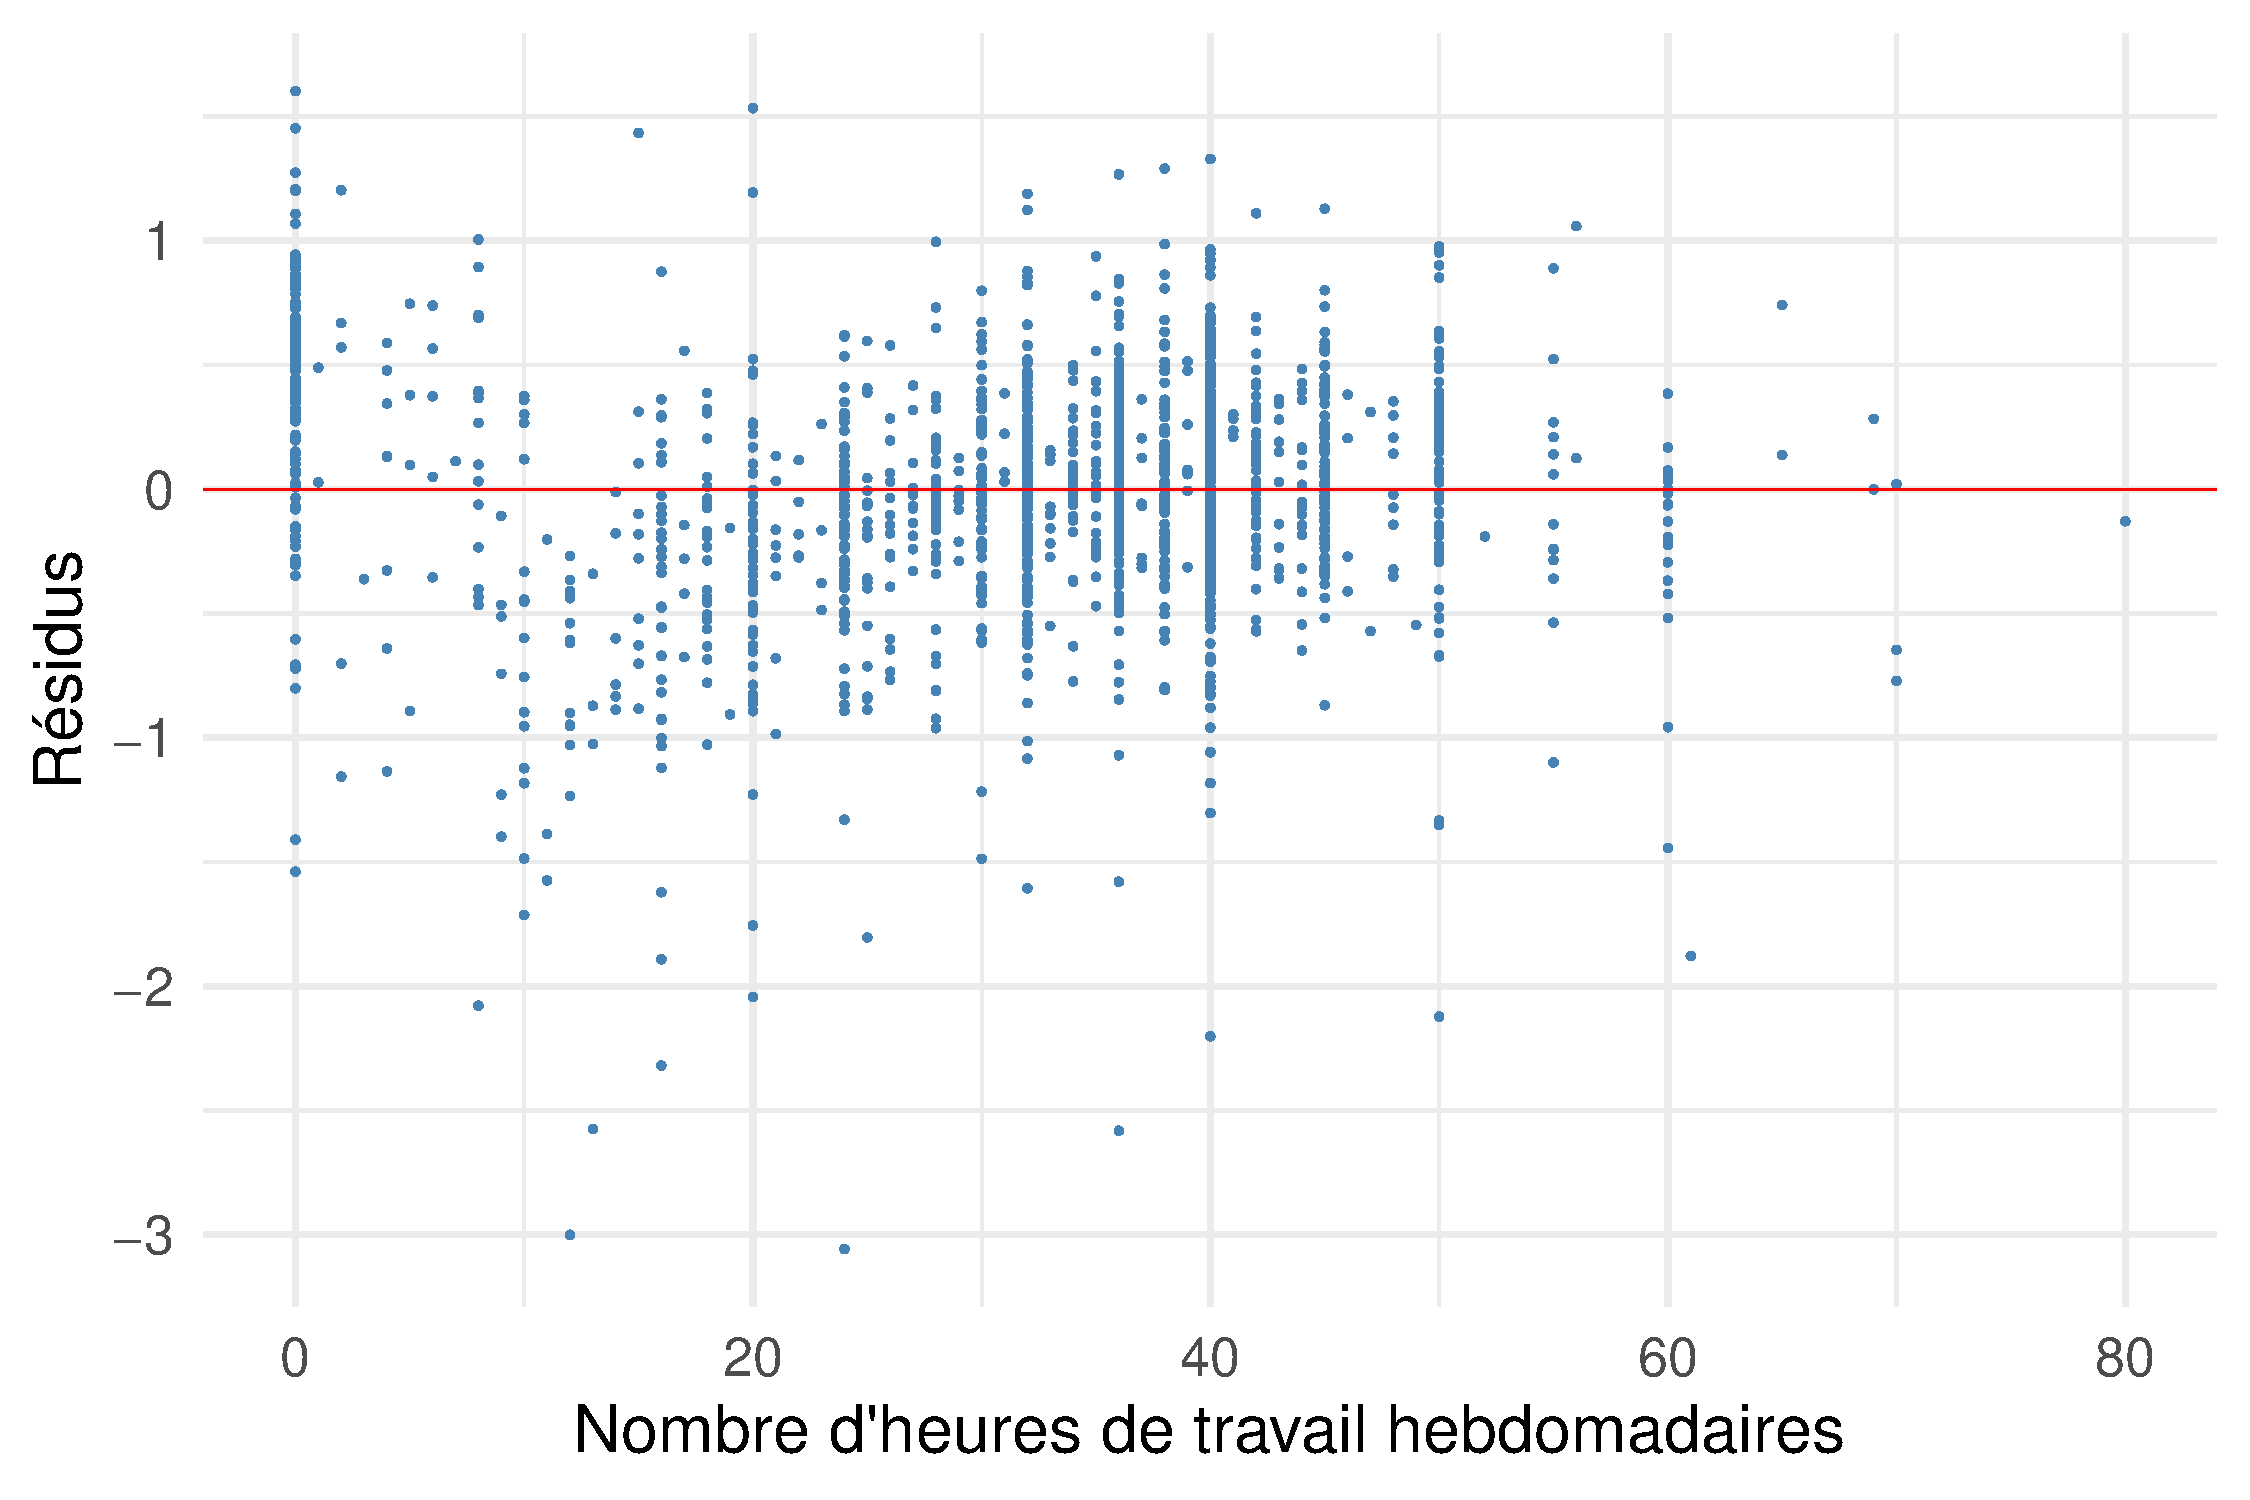
\includegraphics[width=0.49\linewidth]{figure/plot_hetero_heures.pdf}
\caption{Répartition des résidus\label{fig:hetero}}
\end{figure}



Nous avons corrigé l'hétéroscédasticité en utilisant la méthode de white (variante HC1), via la commande \verb+coeftest+. Après correction, nous obtenons le graphique de répartition des résidus suivant, confirmant notre correction avec une variance des résidus d’environ 0,22 pour l’ensemble des observations. Nous remarquons dans la régression linéaire classique que les valeurs des paramètres des régresseurs n’ont pas changé, ces dernières n’étant pas influencées par l’hétéroscédasticité. \ref{fig:hetero_correct}.

\begin{figure}[h]
\center
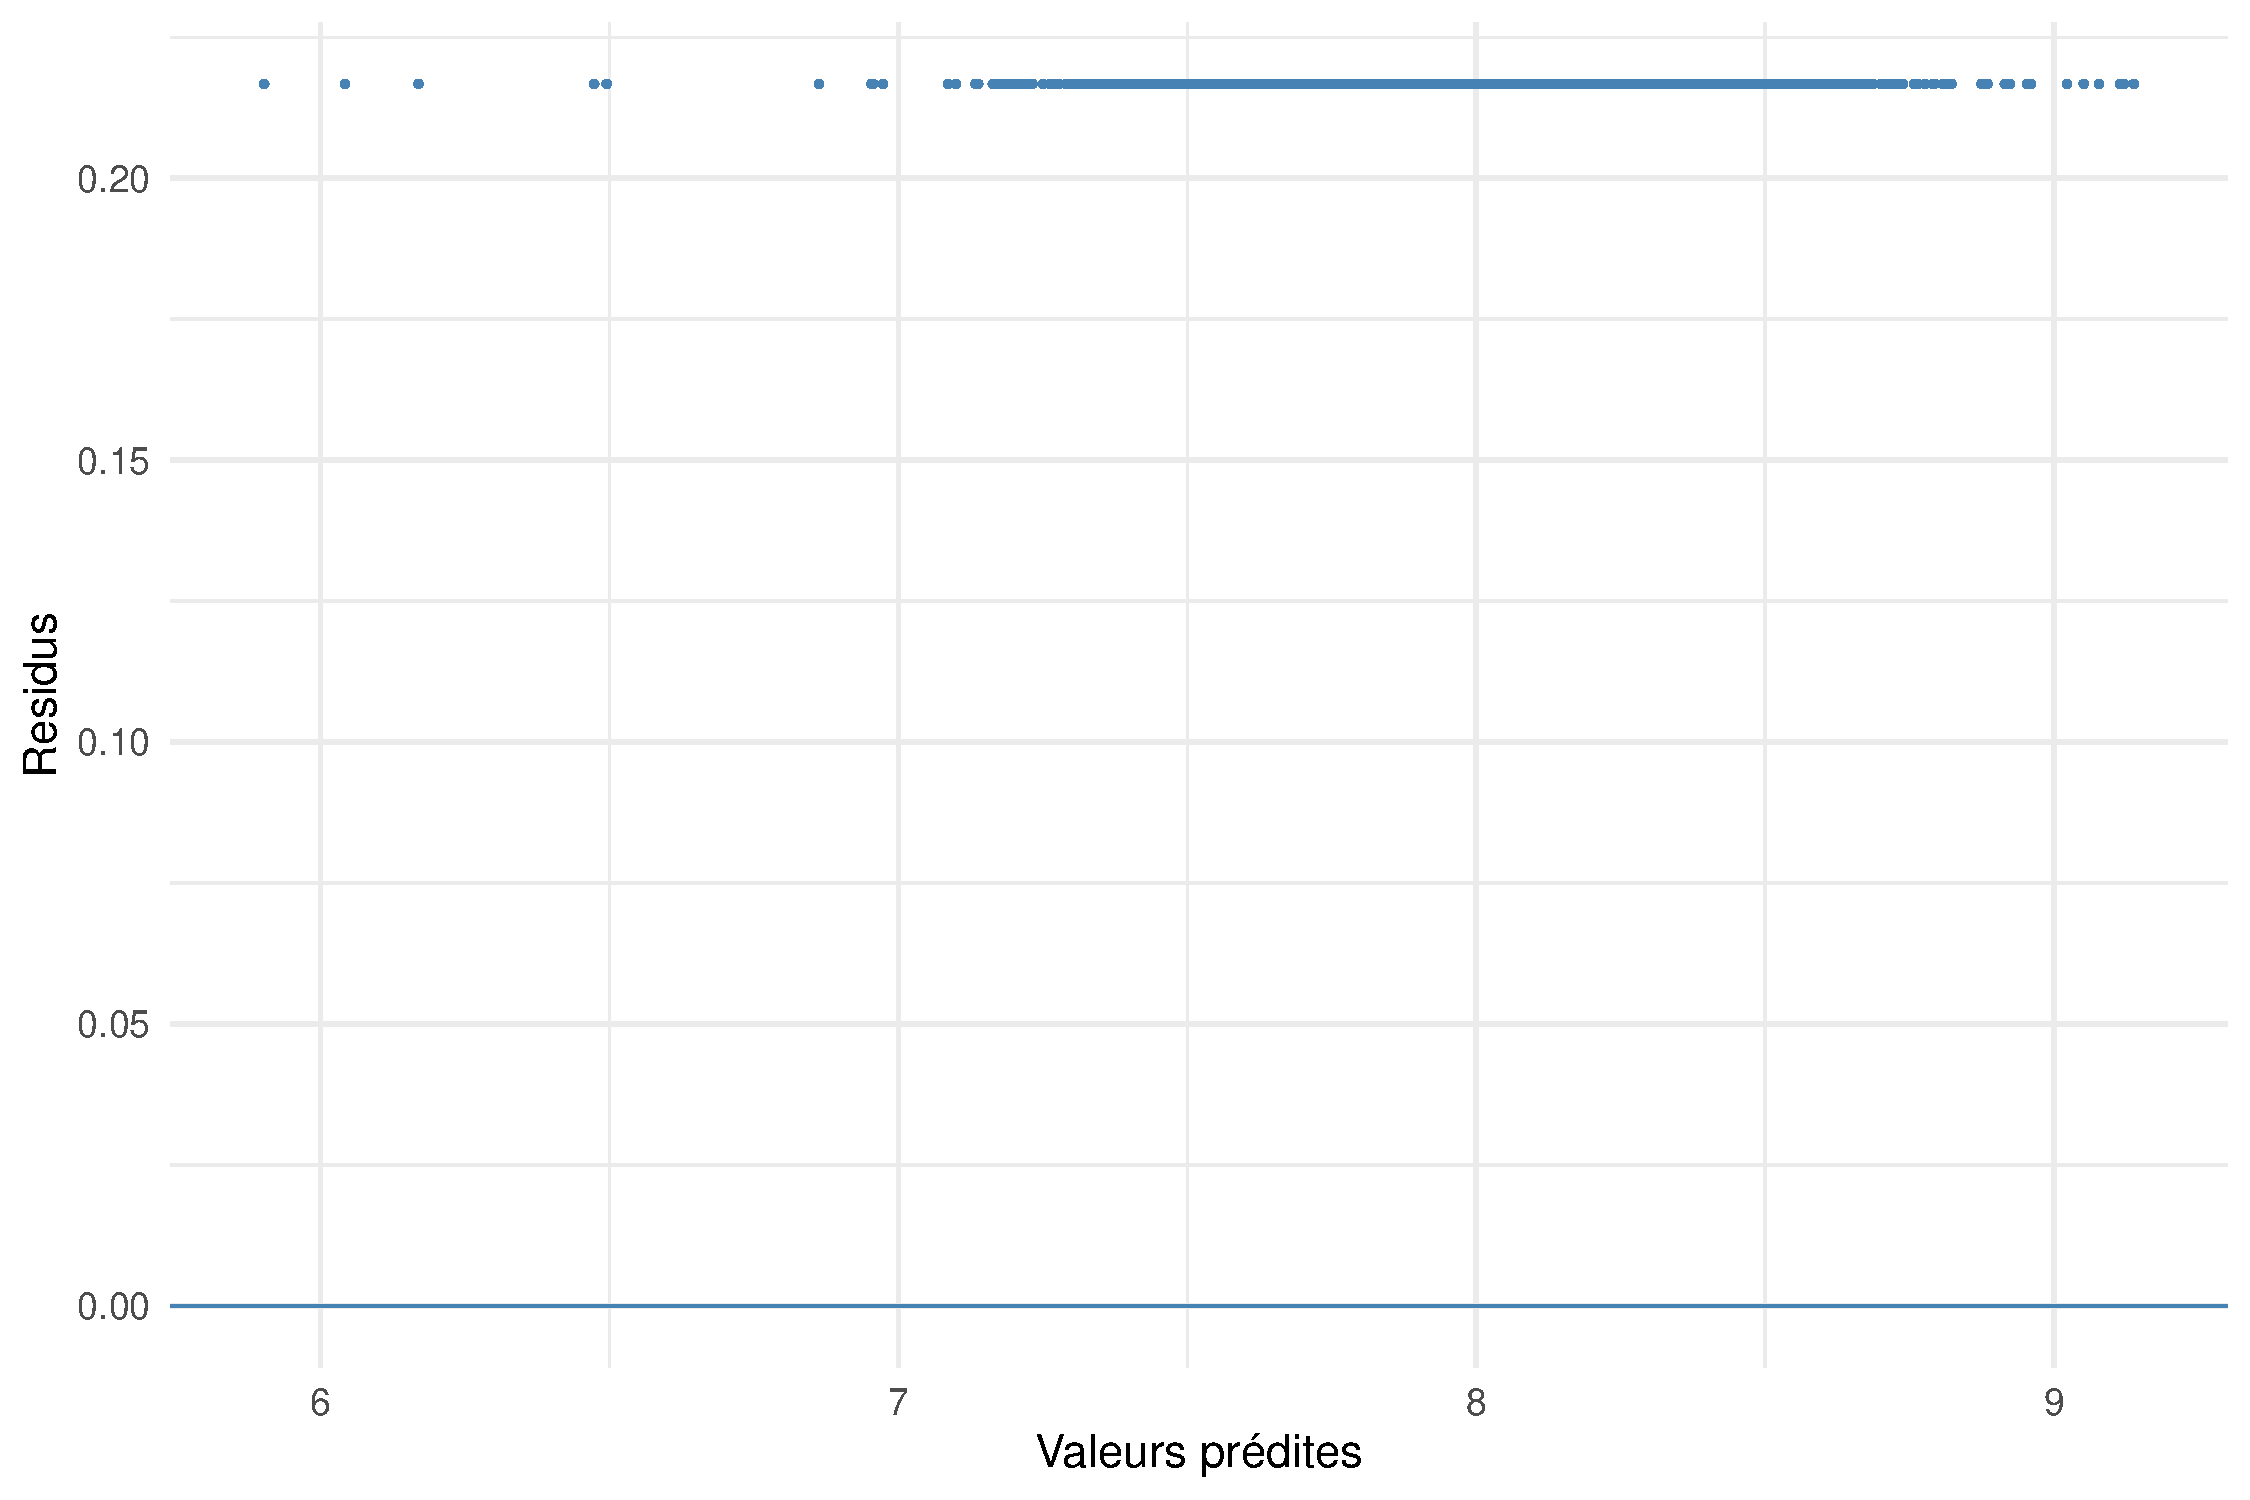
\includegraphics[width=0.7\linewidth]{figure/hetero_correct.pdf}
\caption{Répartition des résidus en fonction des valeurs prédites\label{fig:hetero_correct}}
\end{figure}



\subsection{Détection de l’endogénéité et pistes de correction}

\section{Résultats principaux}

\subsection{Analyse et discussion des paramètres}

% latex table generated in R 4.2.1 by xtable 1.8-4 package
% Mon May 15 22:00:44 2023
\begin{table}[ht]
\centering
\caption{Tableau des résidus} 
\label{tb:lm1}
\begin{tabular}{rrrrr}
  \toprule
 & Estimate & Std. Error & t value & Pr($>$$|$t$|$) \\ 
  \midrule
(Intercept) & 5.8617 & 0.0959 & 61.13 & 0.0000 \\ 
  data\$age & 0.0078 & 0.0010 & 7.77 & 0.0000 \\ 
  data\$genre & -0.3036 & 0.0222 & -13.70 & 0.0000 \\ 
  data\$heures & 0.0140 & 0.0008 & 17.01 & 0.0000 \\ 
  data\$experience & 0.0030 & 0.0011 & 2.65 & 0.0081 \\ 
  data\$nbenfants & -0.0072 & 0.0095 & -0.76 & 0.4483 \\ 
  data\$education & 0.0922 & 0.0046 & 19.93 & 0.0000 \\ 
   \bottomrule
\end{tabular}
\end{table}


Nous avons tout d’abord préféré effectuer une analyse en log-niveau, le log limitant les risques d’hétéroscédasticité en “écrasant” les observations sans les fausser. À première vue, les paramètres de nos 6 régresseurs de base sur la variable expliqués paraissent plutôt cohérents à ce qui est observé dans la littérature, comme le montre le tableau \ref{tb:lm1}, l’âge a une influence positive mais assez négligeable (paramètre de 0,008), le genre a une forte influence négative sur le salaire pour les femmes. Les heures de travail ont évidemment une influence positive forte : 1 heure travaillée en plus par semaine augmente, d’environ 0,14\% le log du revenu (voir figure \ref{fig:heureslogrevenu}).


\begin{knitrout}
\definecolor{shadecolor}{rgb}{0.969, 0.969, 0.969}\color{fgcolor}\begin{kframe}


{\ttfamily\noindent\itshape\color{messagecolor}{\#\# `geom\_smooth()` using formula = 'y \textasciitilde{} x'}}\end{kframe}
\end{knitrout}

\begin{figure}[h]
\center
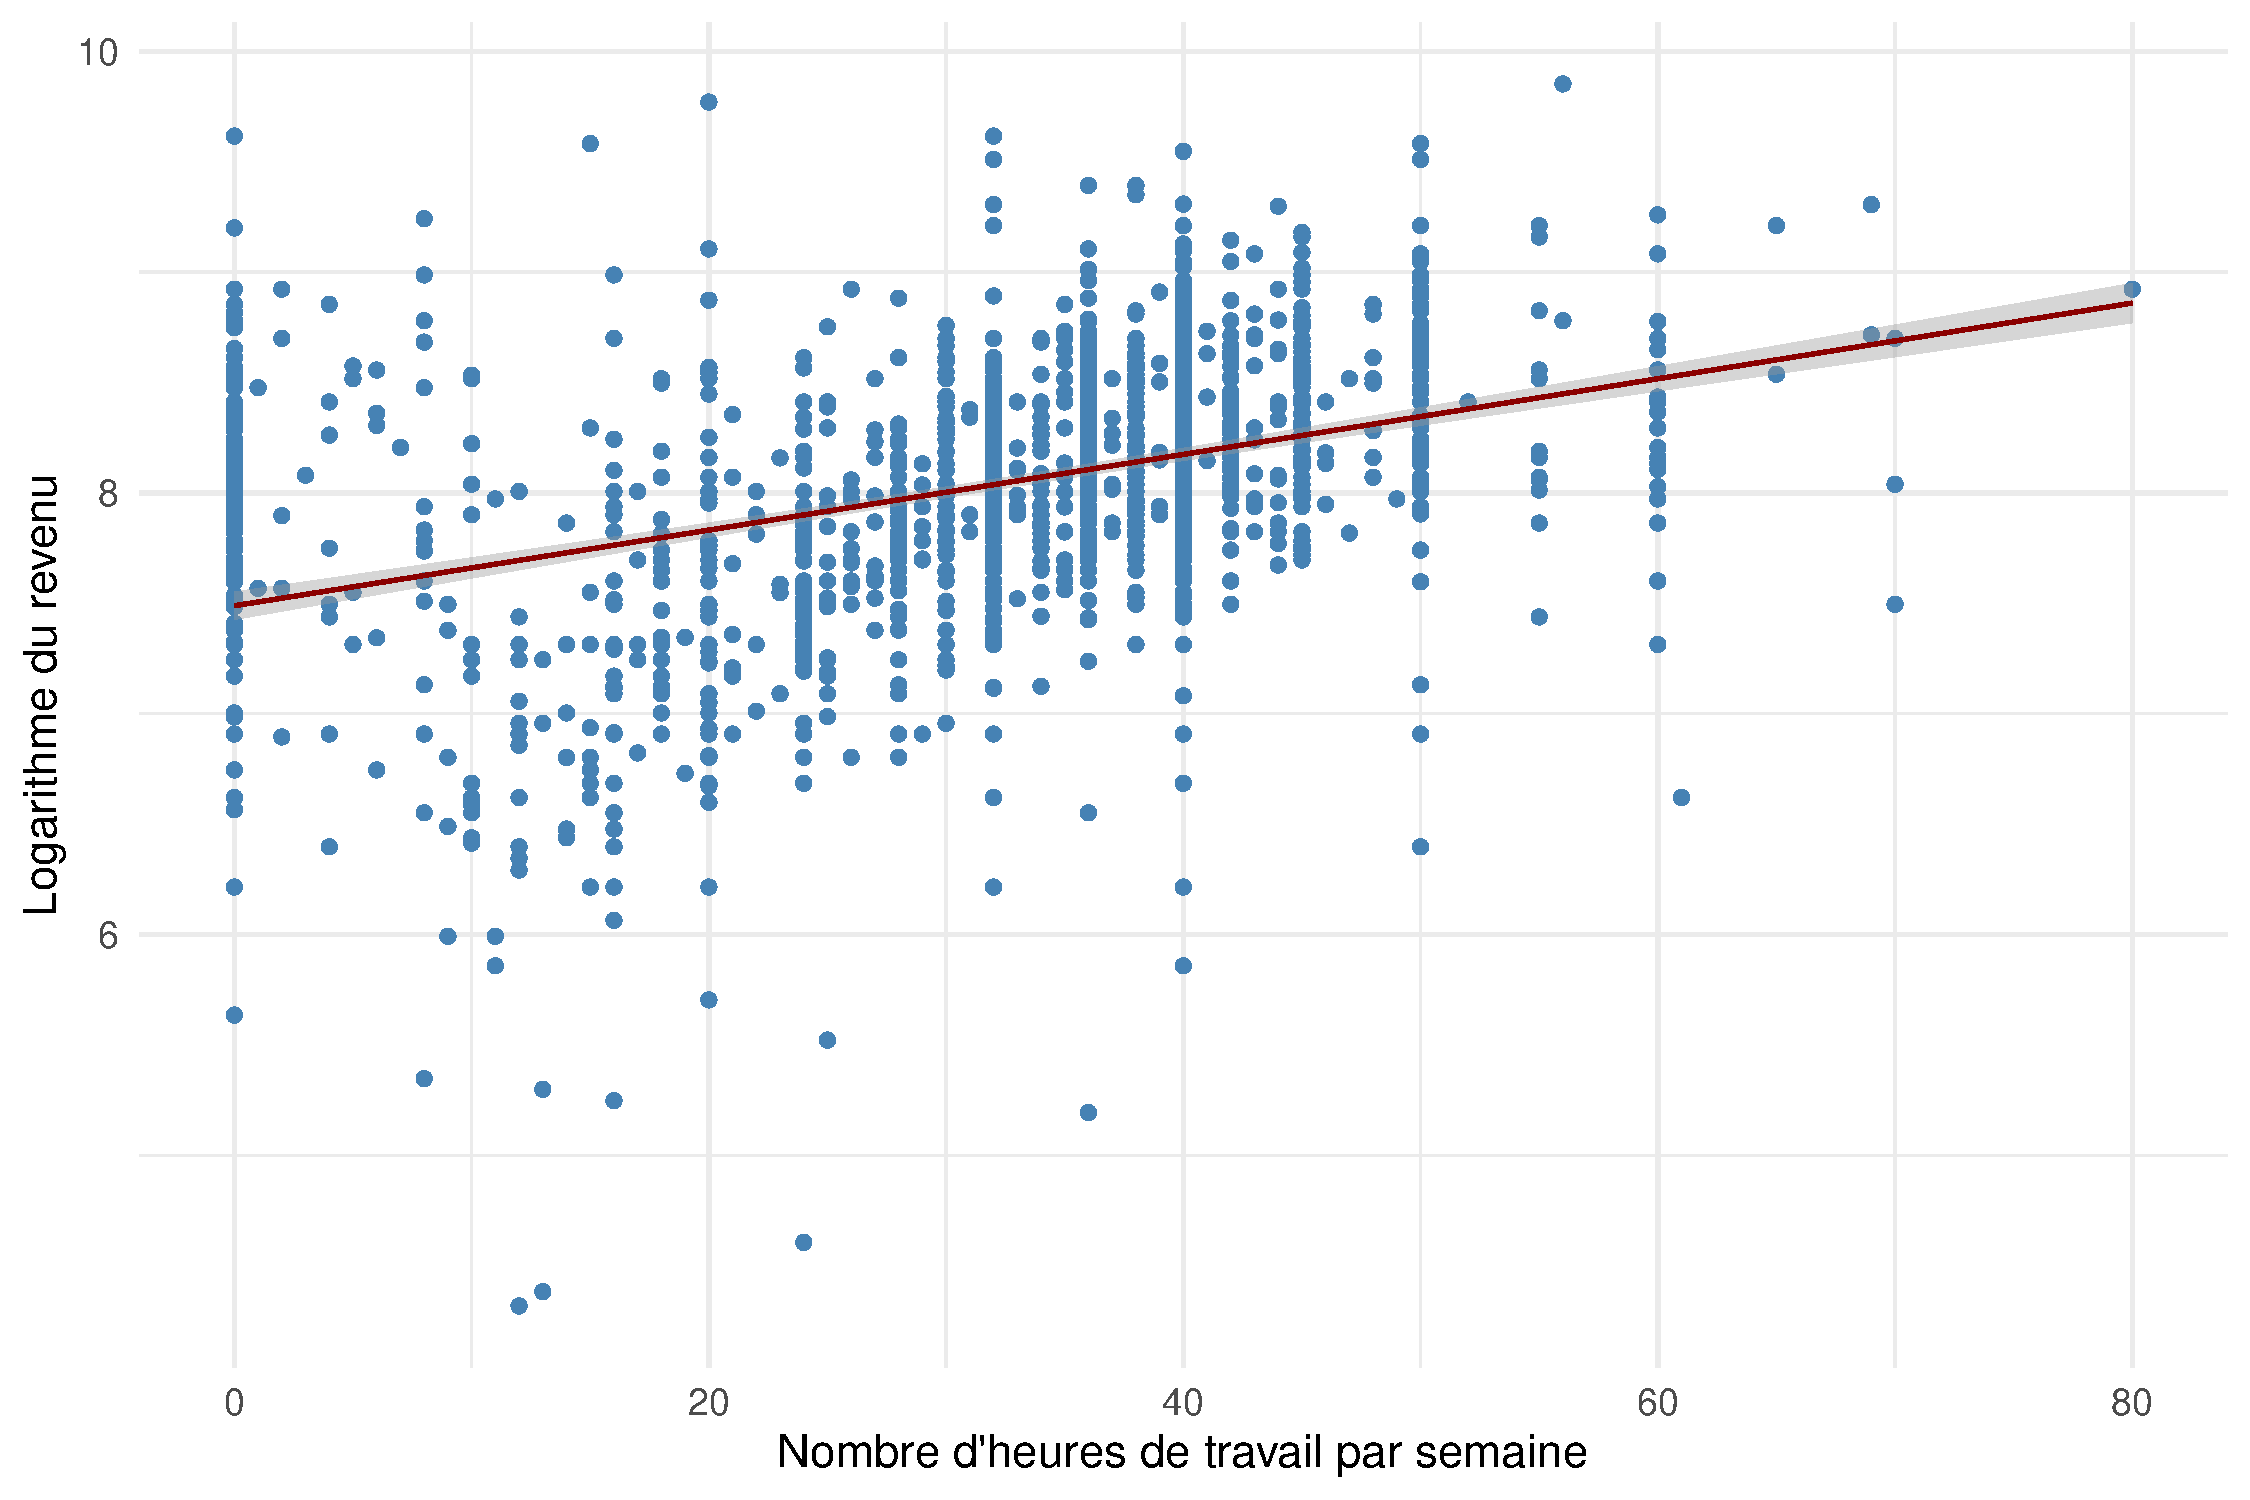
\includegraphics[width=0.7\linewidth]{figure/heures_logrevenu.pdf}
\caption{Log revenu en fonction du nombre d'heures de travail\label{fig:heureslogrevenu}}
\end{figure}

L’expérience joue enfin positivement mais faible, le nombre d’enfants négativement mais faiblement, et l’éducation enfin est la variable qui joue le plus fortement avec le nombre d’heures travaillées, avec un paramètre de 0,09. Fait notable, le nombre d’enfants semble assez peu significatif, cette variable étant la seule dans notre régression initiale avec une p-value supérieure à 0,05 (pour atteindre 0,45).
        Les données du LISS semblent donc confirmer à première vue ce que la littérature a déjà pointé du doigt : une différence structurelle de salaire (brut ici) entre hommes et femmes, une influence positive de l’éducation, de l’expérience, de l’âge… Ayant souhaité nous concentrer plus particulièrement sur l’effet de l’éducation, nous avons cependant souhaité vérifier l’existence d'effets de seuils de l’éducation sur la salaire au moment de l’obtention de diplôme. Nous allons désormais évoquer les résultats d’un test de Chow effectué sur l’éducation. 

\section{Analyse et mise en perspective des résultats}

\subsection{Endogénéité et utilisation de variables instrumentales}

        Une discussion sur la possible présence d’endogénéité dans notre modèle s’impose. Premièrement la variable “éducation” au travers du nombre d’années d’éducation n’est pas exogène. Comme Becker l’avait déjà pointé, tous les individus n’effectuent pas les mêmes choix d’éducation car tous n’ont pas les mêmes ressources pour assumer leurs choix. Une année supplémentaire d’études représente un investissement financier dépendant des ressources à disposition. Par conséquent, au travers du nombre d’années d’étude, c’est probablement également le revenu des parents qui peut se lire. En parallèle, soulignons l’importance et l’influence du parcours scolaire des parents sur celui de leurs enfants, notamment lorsque les parents ont effectué des études supérieures. Des parents diplômés pousseront certainement leurs enfants à faire plus d’études. Une deuxième variable inconnue jouant sur le nombre d’années d’éducation et l’influence sur le salaire indirectement serait donc les ressources disponibles pour l’individu à différents moments de ses études mais aussi le parcours scolaire de ses parents.
        Deuxièmement, l’expérience est évidemment également endogène. Le coefficient de corrélation entre l’âge et l’expérience dans l’entreprise est de 0,52, le plus élevé de tous les coefficients entre variables (soulignons que l’expérience est mesurée comme expérience avec son employeur actuel, une période de chômage remettant cette variable à zéro). Un individu jeune, de 25 ans par exemple, ne pourra évidemment pas accumuler une dizaine d’années d’expérience et au travers de l’expérience, l’âge influe durablement. L’âge est quant à lui une variable exogène par excellence ; à partir de là, prendre l’âge comme variable instrumentale pour corriger l’endogénéité associée à l’expérience pourrait être une option intéressante à tester. Une deuxième source d’endogénéité pesant sur l’expérience serait intéressante à étudier : celle de la formation continue. Ici, la variable éducation se contente d’étudier la durée des études de l’individu, mais qu’en est-il pour ceux qui effectuent, au sein de leur entreprise, une formation complémentaire pour monter en grade ? Ou qui, du fait d’une reconversion professionnelle, effectuent une formation une fois sorti des bancs de l’école ? Un individu avec beaucoup d’expérience a d’autant plus de chances, au cours de ses années passées avec son même employeur, d’avoir effectué une formation complémentaire qui n’est pas prise en compte dans l’éducation mais joue pourtant sur le salaire au travers de l’expérience (nous faisons ici la supposition qu’un individu avec le même employeur depuis longtemps tend statistiquement à plus réaliser de formation en continu, le lien entre stabilité de l’emploi et propension à faire des formations étant confirmé empiriquement).



Et ici on peut écrire ... et insérer des blocs de code qui s'éxécutent, avec le code et le résultat qui s'affichent

\begin{knitrout}
\definecolor{shadecolor}{rgb}{0.969, 0.969, 0.969}\color{fgcolor}\begin{kframe}
\begin{alltt}
\hlstd{a} \hlkwb{<-}  \hlnum{2}\hlopt{+}\hlnum{2}
\hlstd{a}
\end{alltt}
\begin{verbatim}
## [1] 4
\end{verbatim}
\end{kframe}
\end{knitrout}

ou juste le résultat : 

\begin{knitrout}
\definecolor{shadecolor}{rgb}{0.969, 0.969, 0.969}\color{fgcolor}\begin{kframe}
\begin{verbatim}
## [1] 6
\end{verbatim}
\end{kframe}
\end{knitrout}

ou totalement invisibles : 


Et ensuite on peut citer les résultats : à première vue $4 < 6$ mais je crois que c'est 8 qui est le plus grand.





\begin{knitrout}
\definecolor{shadecolor}{rgb}{0.969, 0.969, 0.969}\color{fgcolor}\begin{kframe}
\begin{verbatim}
## [1] 5615
## [1] 0
\end{verbatim}
\end{kframe}
\end{knitrout}



\printbibliography

\appendix
\appendixpage
\addappheadtotoc

\section{Précisions sur les variables utilisées et leur codage}

\subsection{La variable \texttt{age}}

Il s’agit de la variable \texttt{leeftijd}, issue du questionnaire \textit{Background variables}, reprise telle quelle. Les valeurs vont de 16 à 84 ans. 

\subsection{La variable \texttt{education}}

Il s'agit du regroupement de deux variables : nous avons d'abord récupéré les données de la variable \texttt{oplmet} du questionnaire \textit{Background variables} et avons converti les différentes modalités en nombre d'années d'éducation (scolarité et études), comme suit : 

\vspace{0,5cm}
\begin{minipage}{0,8\linewidth}
{\footnotesize\texttt{oplmet} : Highest level of education with diploma
\vspace{0,2cm}

\begin{tabular}{m{0,5\linewidth}m{0,5\linewidth}}
\hline
Valeur d'origine & Valeur de remplacement \\
\hline
1. primary school [8 ans] & 8 (de 4 à 12 ans) \\
2. vmbo (intermediate secondary education, US: junior high school) [4 ans] & 12 (après l'école primaire) \\
3. havo/vwo (higher secondary education/preparatory university education, US: senior high school) [5-6 ans] & 13.5 (après l'école primaire) \\
4. mbo (intermediate vocational education, US: junior college) [1-4 ans] & 15.25 (après VMBO, HAVO ou VWO, soit en moyenne 2.5 + 12.75)\\
5. hbo (higher vocational education, US: college)[4 ans] & 16.75 (après VMBO, HAVO ou VWO, 4 + 12.75)\\
6. wo (university) [3 ans]& 17 (après 1ere année HBO ou après VWO, 14 + 3)\\
7. other & suppression des observations \\
8. Not (yet) completed any education & 0 \\
9. Not yet started any education & 0 \\
\hline
\end{tabular}}
\end{minipage}
\vspace{0,3cm}

La variable \texttt{oplmet} ne proposant pas de modalité \textit{master} ou \textit{Ph.D.}, nous nous sommes ensuite appuyés sur la variable \texttt{cw22o005} du questionnaire \textit{Work and schooling}. Cette variable, très complète, comprend 28 modalités, ce qui la rendait trop difficile à coder étant donné que nous ne maîtrisons pas les subtilités du système universitaire néerlandais, mais nous nous sommes contentés de récupérer les trois modalités qui nous intéressent, afin de compléter le codage de la variable \texttt{education}, comme suit : 

\vspace{0,5cm}
\begin{minipage}{0,8\linewidth}
{\footnotesize\texttt{cw22o005} : What is the highest level of education that you have completed with diploma or certificate?
\vspace{0,2cm}

\begin{tabular}{m{0,5\linewidth}m{0,5\linewidth}}
\hline
Valeur d'origine & Valeur de remplacement \\
\hline
25. academic education, bachelor [3 ans] & 17 (soit la valeur que nous avions déjà) \\
26. academic education, master [1-3 ans] & 19 (17 +2) \\
27. doctor's degree (Ph.D, including doctoral research program to obtain Ph.D) [3-4 ans] & 22.5 (19+3.5) \\
\hline
\end{tabular}}
\end{minipage}

À l'issue du codage, on obtient la répartition suivante : 

\begin{figure}[h]
\center
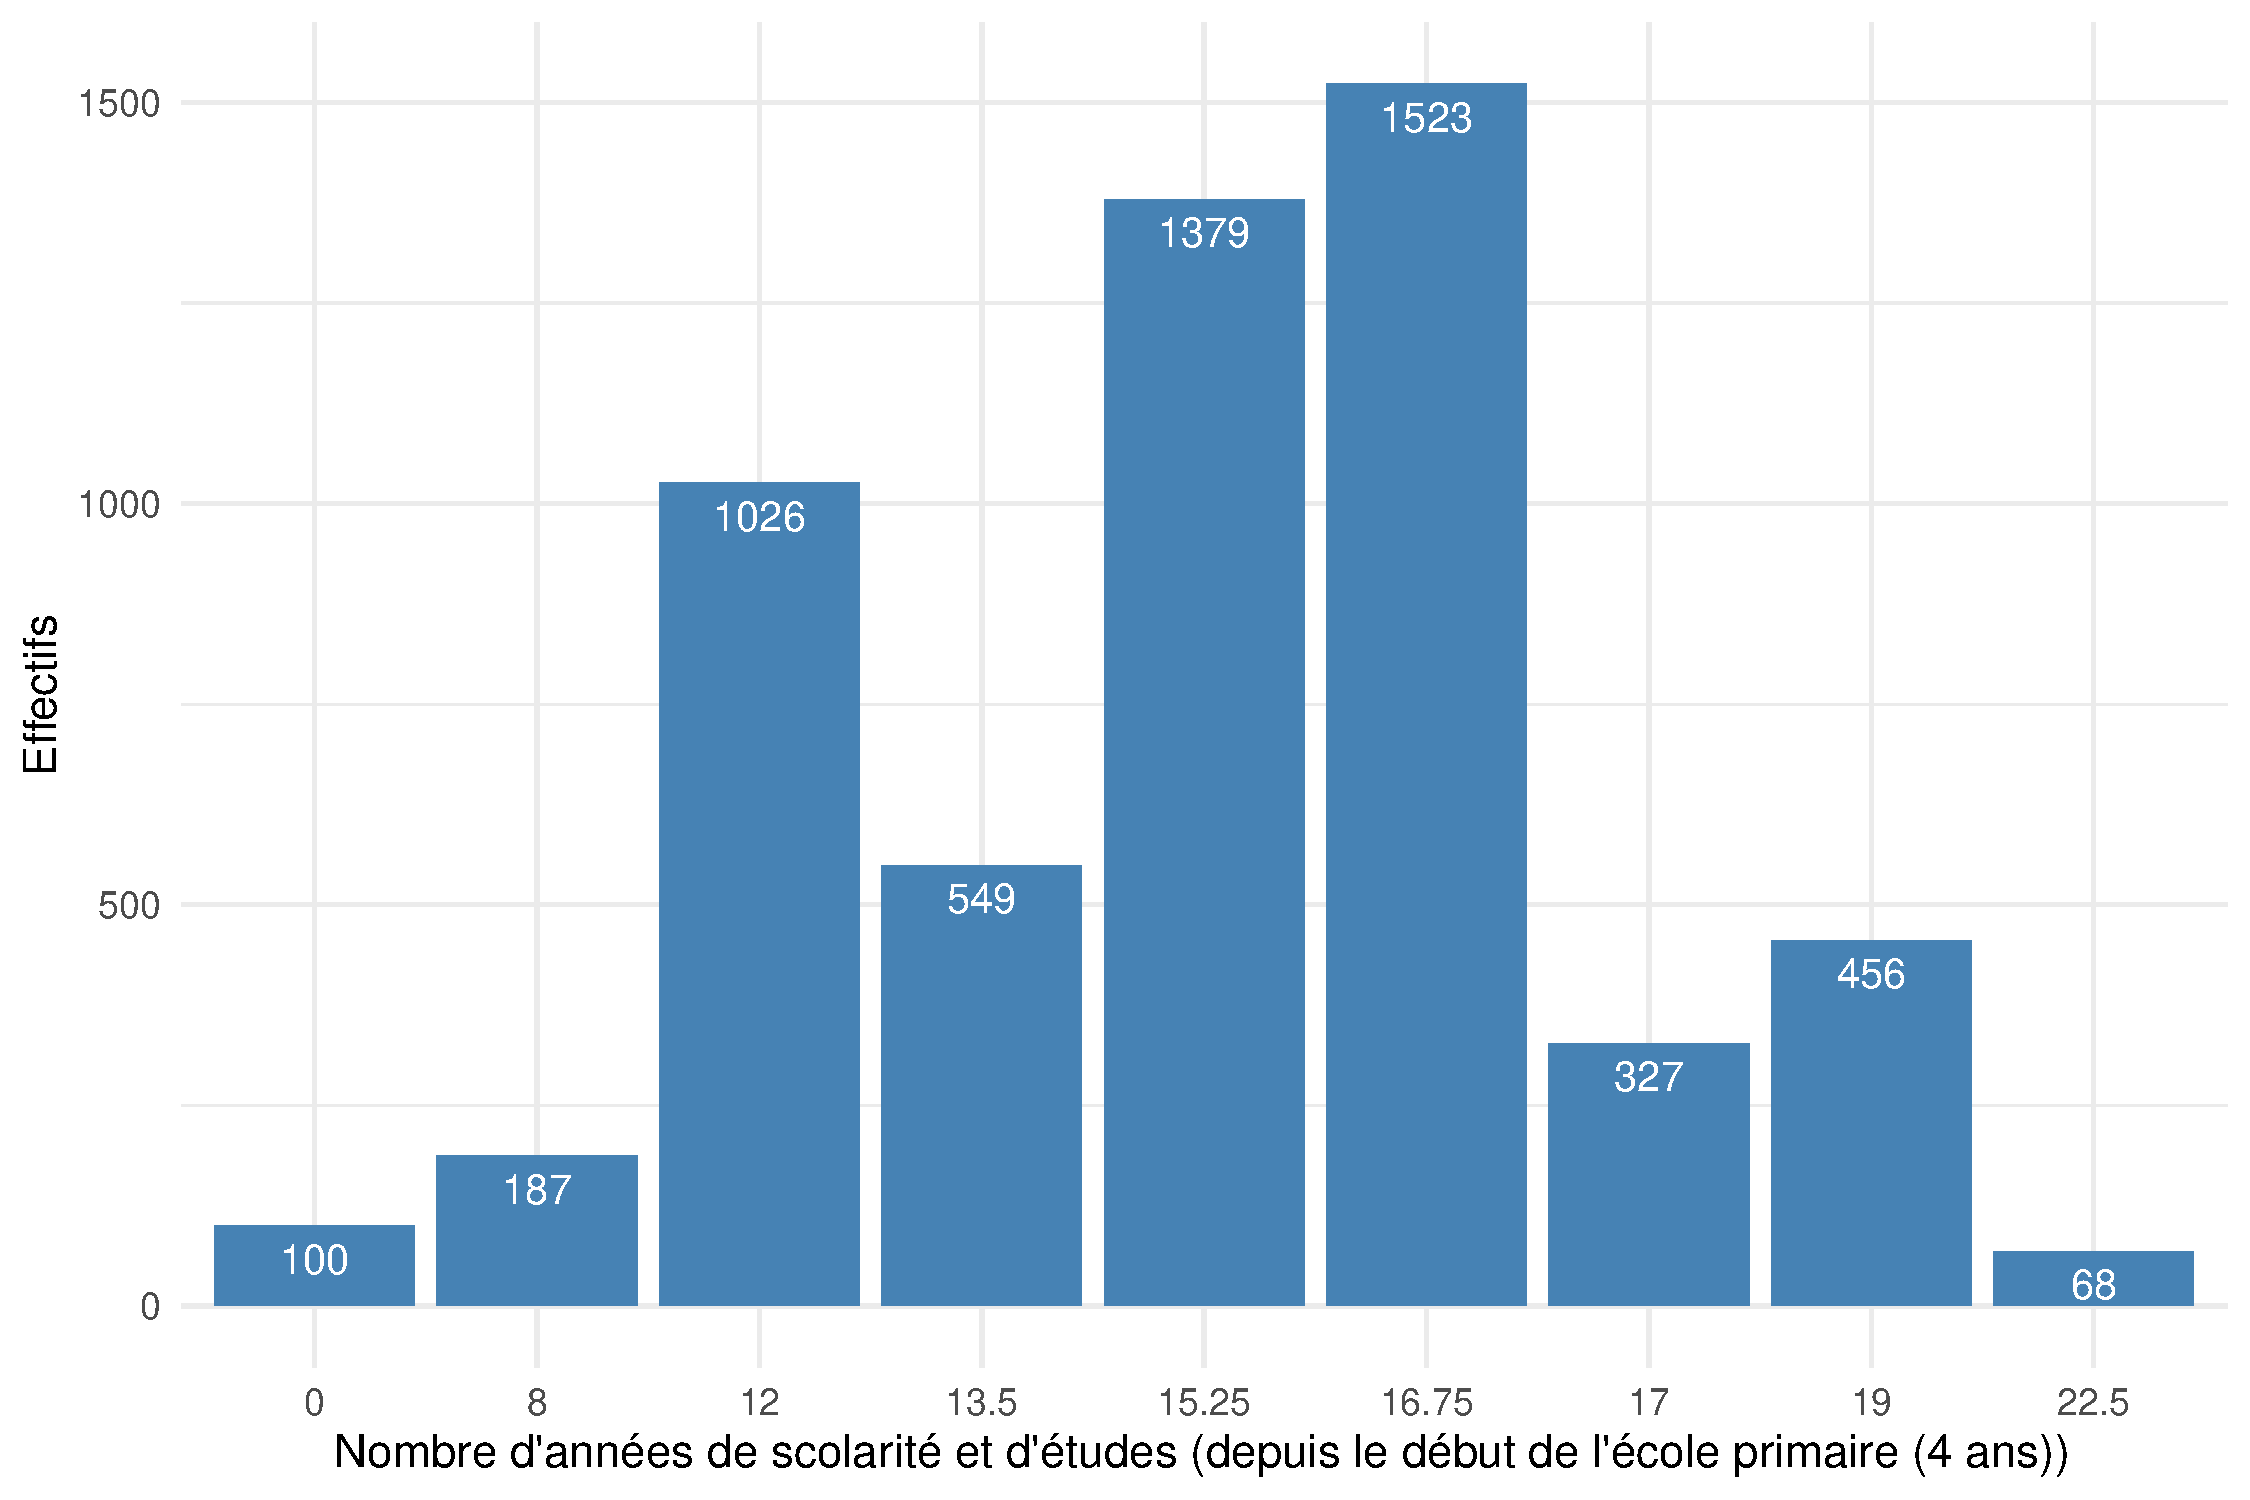
\includegraphics[width=0.7\linewidth]{figure/educ.pdf}
\caption{Niveau d'éducation (avec diplôme) des individus de l'échantillon}
\end{figure}

\subsection{La variable genre}

Cette variable est issue de la variable \texttt{geslacht} du questionnaire \textit{Background variables}, dont nous avons enlevé toutes les réponses autres (ni masculin, ni féminin), qui sont par ailleurs très minoritaires (4 observations, soit moins de 0,1\% des observations)

\subsection{La variable revenu}

Issue de la variable \texttt{brutoink} du questionnaire \textit{Background variables}, elle correspond au revenu brut mensuel individuel (\textit{personal gross monthly income}), dans notre modèle, nous utilisons principalement le logarithme de cette variable (\verb+log_revenu+). Nous avons décidé de supprimer les observations pour lesquelles le revenu déclaré est nul, suivant l'avertissement présent dans le \textit{codebook} du LISS : 

\begin{quote}
\textcolor{gray}{Since some people prefer not to make their income information available to Centerdata, a 0 (zero) can mean two different things: (1) that there is no income at all, or (2) that a panel member does not know what the income is or does not want to make that information available to us.}
\end{quote}

\subsection{La variable heures}

Il s'agit de la variable \texttt{cw22o127} du questionnaire \textit{Work and schooling}, qui correspond à la question : \enquote{How many hours per week do you work on average? / How many hours per week did you work on average?}, que nous avons reprise telle quelle. Les valeurs s'échelonnent de 0 à 80 heures hebdomadaires, avec une médiane égale à 36 heures.

\subsection{La variable \texttt{experience}}

Issue du questionnaire \textit{Work and schooling} (variable \texttt{cw22o134}), il s'agit de la réponse à la question : \enquote{In which year did you enter into employment with your current employer?}. Nous n'avons appliqué aucun traitement particulier aux observations, en dehors de la suppression des \textit{NA}.Les valeurs vont de 0 à 58 ans d'ancienneté, avec une médiane à 7 ans et une moyenne à 12 années d'ancienneté. 

\subsection{La variable \texttt{nbenfants}}

Issue de l'enquête \textit{Background variables}, il s'agit du nombre d'enfants vivant au sein du foyer (\enquote{Number of living-at-home children in the household, children of the household head or his/her partner}). Nous l'avons reprise sans modifier ses valeurs. 

\end{document}
